\section{Probabilistic Co-Design Metrics: Formalizing the Refinement vs. Realization Trade-Off}\label{sec:apx:holisticcodesign:probabilistic_co_design_metrics}
% As introduced earlier, in our proposed holistic co-design framework, there exists an inherent trade-off between refinement vs. realization in the setting where we take a probabilistic perspective on evaluation metrics, such as manufacturability or task-centric performance.
% Then, refinement refers to executing a computational co-design cycle that includes both the evaluation of (a) new design candidate(s) and subsequently updating the posterior design sample policy based on the current evaluation metric prior.
% On the other hand, realization refers to increasing our certainty in the metric by running high-fidelity simulations and/or building prototypes with increasing TR-Ls.
As discussed earlier, our holistic co-design framework inherently balances a trade-off between refinement and realization when evaluation metrics—such as manufacturability or task-centric performance—are treated probabilistically. In this setting, refinement involves running a computational co-design cycle that evaluates new design candidate(s) and updates the posterior design sampling policy based on the current evaluation metric prior. Conversely, realization seeks to enhance our confidence in the metric by performing high-fidelity simulations and/or fabricating prototypes with progressively higher \glspl{TRL}~\citep{junge2022leveraging}.

To formalize this further, consider an evaluation metric $c_j = m_j(x)$ that assigns a cost $c_j \in \mathcal{C}_j$ to a design $x \in \mathcal{X}$, which we aim to minimize during the co-design process. 
Here, the subscript $j$ indicates the $j$th metric and its associated cost $c_j$.
As noted earlier, the soft robot co-design problem is typically addressed in a multi-objective context where various metrics capture aspects such as task performance (e.g., task completion time, energy consumption), safety, controllability, observability, manufacturing costs, and more. 
In practice, however, accurately evaluating these metrics is typically very expensive since it involves building a prototype and conducting extensive field trials or user studies. Instead, we may have access to a simplified computational model or a current probabilistic belief about the metric, denoted as $\hat{m}_j(\hat{c}_j, x): \mathcal{C}_j \times \mathcal{X} \to [0,1]$,
which maps a design $x$ and an estimated cost\footnote{The cost is equivalent to a loss and may also be viewed as a negative reward.} $\hat{c}_j \in \mathcal{C}_j$ to a probability $\mathrm{Pr}(\hat{c}_j,x)$.
We now detail the definitions of refinement and realization in this framework.

\begin{figure}[ht]
    \centering
    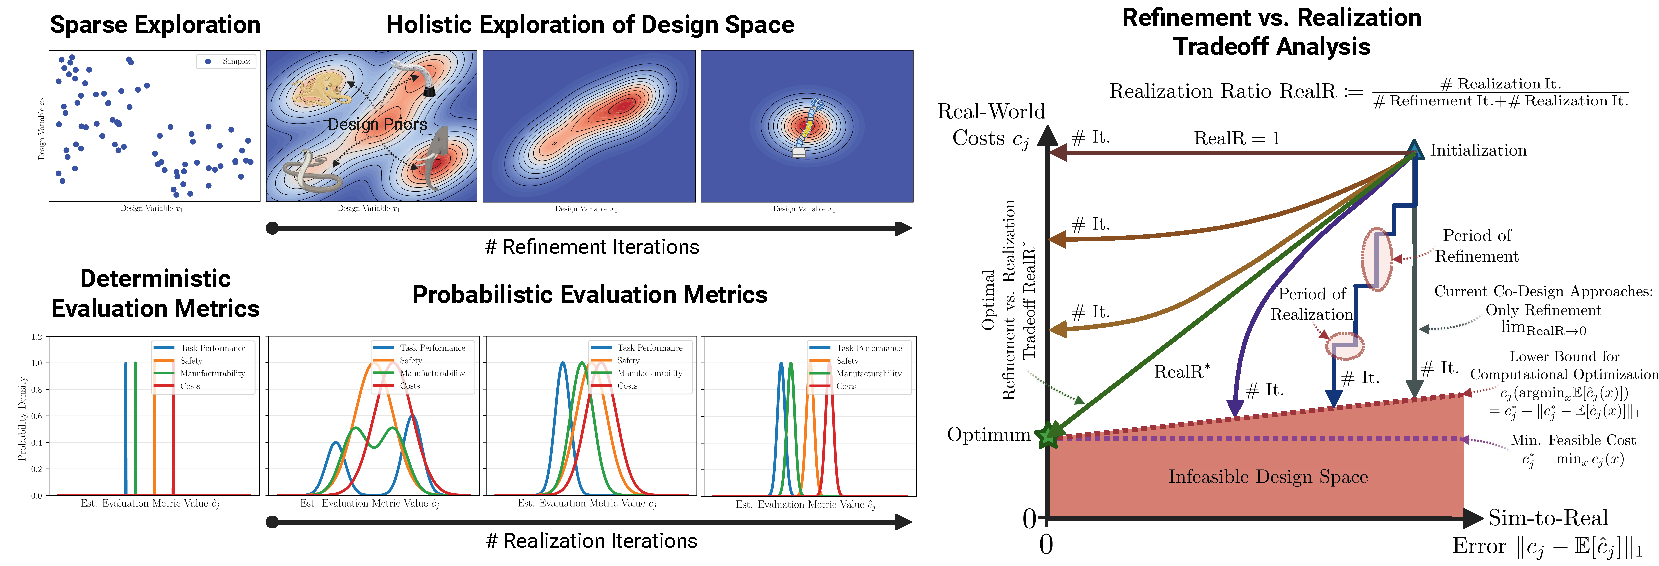
\includegraphics[width=1.0\linewidth]{appendix-holistic-codesign/figures/refinement_vs_realization_tradeoff_optimized.pdf}
    \caption{\textbf{Refinement vs. Realization.}
    \textit{Top Left:} This panel shows how refinement affects the design sampling distribution $\vartheta(x)$. Unlike (most) conventional co‑design methods that sparsely explore the design space, we condition $\vartheta(x)$ on design priors (e.g., biological inspiration and existing soft robot designs) and iteratively update it via the co‑design optimizer until the optimum is reached.
    \textit{Bottom Left:} Here, we demonstrate how iterative realization refines probabilistic evaluation metrics. Rather than using deterministic metrics that ignore inherent simulation uncertainty, we define a probabilistic distribution $\hat{m}_j(\hat{c}_j, x)$ for each metric, with purposeful prototyping reducing the uncertainty over iterations.
    \textit{Right:} This panel examines the tradeoff between refinement and realization. We define the realization ratio $\mathrm{RealR}$ as the fraction of realization iterations relative to the total iterations and the sim‑to‑real error as $\lVert c_j - \mathbb{E}[\hat{c}_j] \rVert$. We then plot the evolution of real-world cost $c_j$ versus sim‑to‑real error as iterations increase for a fixed $\mathrm{RealR}$: when $\lim{\mathrm{RealR} \to 0}$, designs are optimized computationally with realization occurring only at the end, while $\mathrm{RealR}=1$ means only the confidence in the evaluation metrics is increased. The optimal ratio $\mathrm{RealR}^*$ efficiently minimizes the real-world cost to its optimum $\min_x c_j(x)$ via refinement and reduces the sim‑to‑real error to zero by updating $\hat{m}_j(\hat{c}_j, x)$ via realization.
    }\label{fig:apx:holisticcodesign:refinement_vs_realization_tradeoff}
\end{figure}

\textbf{Refinement.}
During refinement, we adopt a Monte Carlo procedure by querying the metric conditioned on the design, i.e., $\hat{c}_j \sim m_j(\cdot, x)$. The resulting estimated cost $\hat{c}_j$ is then employed either as an optimization objective or as part of a constraint. Crucially, the optimizer leverages this estimated cost to update the posterior distribution of the design variables $x$, adjust any free parameters of the decoder $\vartheta(x)$, and tune other pertinent parameters such as control or observer gains or hyperparameters of the reduced-order model. This process represents one iteration of computational co-design, which can be visualized as one cycle in Fig.~\ref{fig:apx:holisticcodesign:computational_co_design} and as a cycle within the innermost layer in Fig.~\ref{fig:apx:holisticcodesign:current_design_vs_holistic_codesign}~(Right). Drawing an analogy to traditional product development cycles, refinement resembles the \emph{diverging} phase, where new concepts and designs are explored and assessed. Similarly, during \emph{exploitation} phases in RL, where a fixed action policy $\pi(a,s)$ is followed during inference without necessarily updating the policy's parameters. In our context, instead of a reward for following the action policy, our outcome is a posterior design generator distribution along with updated design decoder parameters.

\textbf{Realization.}
In realization, our goal is to boost our confidence in the defined metrics. Specifically, we aim to maximize the expected information gain regarding the metrics for the current best design—effectively reducing the entropy (or uncertainty) of the metric’s posterior around the optimal design. To do this, we can employ methods like Predictive Entropy Search (PES) from Bayesian optimization~\citep{hernandez2014predictive}, which assists in pinpointing the global minimizer $x^*$ of the $j$th cost $c_j$. The acquisition function $\alpha_\mathrm{PES}(x): \mathcal{X} \to \mathcal{C}_j$ then enables us to select the next candidate point
$x_\mathrm{n} = \arg \min_{x \in \mathcal{X}} \, \alpha_\mathrm{PES}(x)$
that most effectively reduces the uncertainty regarding the location of $x^*$~\citep{hernandez2014predictive}, where
\begin{equation}
    \alpha_\mathrm{PES}(x) = H[\hat{m}_j(x)] - \mathbb{E}_{\hat{m}_j(x^*)} \left[ H\big(\mathrm{Pr}(\hat{c}_j \mid x,x^*)\big) \right],
\end{equation}
and $H[p(x)] = -\int p(x) \log(p(x)) \, \mathrm{d}x$ denotes the differential entropy. 
% An additional challenge in holistic co-design lies in the fact that we do not just strive to minimize the uncertainty with respect to the optimimum of one metric via realization, but instead for all metrics part of the multi-objective optimization problem. Therefore, an emphasis of future research should lie on techniques that can best select the next sample point $x_\mathrm{n}$ for realization that simultaneously minimizes uncertainty of many/all metric estimates $\hat{m}_j$ while reducing/taking into account the cost, time, and effort needed to obtain the ground-truth measurements for the metrics.
Another challenge in holistic co-design is that our goal is not only to reduce uncertainty about the optimum of a single metric through realization but to do so for all metrics involved in the multi-objective optimization problem. Consequently, future research should focus on developing methods that effectively select the next sample point $x_\mathrm{n}$ for realization, simultaneously minimizing the uncertainty across multiple metric estimates $\hat{m}_j(x_\mathrm{n})$ while also accounting for the cost, time, and effort required to obtain accurate ground-truth measurements.
We conclude that in holistic co-design, realization aligns with the \emph{converging} phases of traditional product development, where concepts and designs are validated through simulations or prototypes to reduce risk and uncertainty, thereby informing better future decisions (for instance, by ruling out designs that are suboptimal based on more certain metrics). Similarly, just as \gls{RL} utilizes random policies to explore unseen state-action pairs~\citep{sutton1998reinforcement} within \emph{exploration} phases\footnote{A key difference between exploration in \gls{RL} and realization in co-design is that in product development, the final optimized system must be implemented, whereas in \gls{RL}, further exploration may be unnecessary if the policy already meets performance expectations.}, we advocate leveraging high-fidelity simulators and prototypes to verify and enhance metrics for previously untested designs.

In practice, it is crucial to strike a balance between refinement and realization, similar to the exploitation vs. exploration tradeoff in RL. Refinement can generate (potentially) better designs at the cost of computational time, and the resulting design may not be optimal due to uncertainties in the predicted costs of the various metrics—essentially, a discrepancy between model predictions and reality. In contrast, realization does not directly enhance the design; instead, it bolsters our confidence in the metrics through high-fidelity simulations and prototyping tests at different \glspl{TRL}, often incurring significant expense, particularly when human designers are involved in fabricating and validating the prototypes. To manage this trade-off, established techniques from \gls{RL}~\citep{sutton1998reinforcement} and Bayesian optimization~\citep{garnett2023bayesian} can be applied. For example, one viable approach is to assess the Expected Improvement (EI)~\citep{jones1998efficient} when sampling a new design and building its prototype while accounting for the uncertainty inherent in the metric under consideration.

Even when a balance between refinement and realization is achieved, realization—through prototyping and real-world validation—remains both resource- and cost-intensive. To address this challenge, we propose that the community create a shared database where researchers and engineers can contribute soft robotic designs along with their performance benchmarks. In line with efforts to enhance soft robot benchmarking~\citep{bhatia2021evolution, wang2023softzoo} and reproducibility~\citep{baines2024need}, such a repository would improve the initial probabilistic beliefs in the metrics and reduce uncertainty in computational evaluations. Ultimately, this would lessen the reliance on expensive realization processes, which is especially important for aspects like serial production costs that are impractical to repeat multiple times during a given design cycle.